\documentclass[a4paper,12pt]{book}
\usepackage[utf8]{inputenc}
\title{}
\author{Rachel Morris}
\date{\today}

\usepackage{rachwidgets}
\usepackage{fancyhdr}
\usepackage{lastpage}
\usepackage{dirtree}
\usepackage{boxedminipage}

\setcounter{chapter}{7}
\setcounter{section}{2}
\newcommand{\laChapter}{7.3 Isomorphism and Planarity\ }

\newcommand{\laClass}{CS 211\ }
\newcommand{\laSemester}{Fall 2017\ }
\newcounter{question}

\pagestyle{fancy}
\fancyhf{}
\lhead{\laClass Exercise, \laSemester}
\chead{}
\rhead{Ch \laChapter}
\rfoot{\thepage\ of \pageref{LastPage}}
\lfoot{\scriptsize Compiled by Rachel Morris, last updated \today}

\renewcommand{\headrulewidth}{2pt}
\renewcommand{\footrulewidth}{1pt}

\begin{document}

    %\toggletrue{answerkey}
    \togglefalse{answerkey}

    \notonkey{

    %- Team Info ------------------------------------------------------%

    Please write down all people in your team. ~\\

    % table %
    \begin{tabular}{ p{6cm} p{6cm} }
        1. & 2. \\ \\
        3. & 4.
    \end{tabular}
    % table %
    ~\\

    \hrulefill
    }{}

    \section*{Review: Functions}

    \notonkey{

    \begin{introNOHEAD}{}
        \paragraph{Properties of Functions}
        \begin{wrapfigure}{r}{0.3\textwidth}
            \begin{center}
                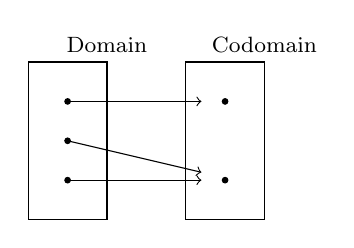
\begin{tikzpicture}
                    \draw (0, 0) rectangle (1, 2) node[above] {\footnotesize Domain};
                    \draw (2, 0) rectangle (3, 2) node[above] {\footnotesize Codomain};
                    \filldraw (0.5, 0.5) circle (1pt);
                    \filldraw (0.5, 1) circle (1pt);
                    \filldraw (0.5, 1.5) circle (1pt);
                    \filldraw (2.5, 0.5) circle (1pt);
                    \filldraw (2.5, 1.5) circle (1pt);
                    \draw[->] (0.5, 0.5) -- (2.2, 0.5);
                    \draw[->] (0.5, 1) -- (2.2, 0.6);
                    \draw[->] (0.5, 1.5) -- (2.2, 1.5);
                \end{tikzpicture}
                \footnotesize Onto but not one-to-one
            \end{center}
            
            \begin{center}
                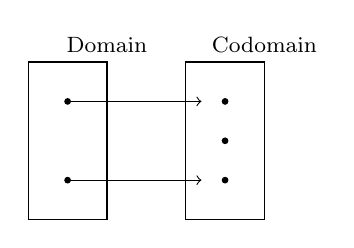
\begin{tikzpicture}
                    \draw (0, 0) rectangle (1, 2) node[above] {\footnotesize Domain};
                    \draw (2, 0) rectangle (3, 2) node[above] {\footnotesize Codomain};
                    \filldraw (0.5, 0.5) circle (1pt);
                    \filldraw (0.5, 1.5) circle (1pt);
                    \filldraw (2.5, 0.5) circle (1pt);
                    \filldraw (2.5, 1) circle (1pt);
                    \filldraw (2.5, 1.5) circle (1pt);
                    \draw[->] (0.5, 0.5) -- (2.2, 0.5);
                    \draw[->] (0.5, 1.5) -- (2.2, 1.5);
                \end{tikzpicture}
                \footnotesize One-to-one but not onto
            \end{center}
        \end{wrapfigure}

        \begin{itemize}
            \item   \textbf{Onto:}
                    A function is \textbf{onto} if every element of
                    the codomain has at least one element in the
                    domain pointing to it. (Every output is attainable
                    via at least one input.)

                    
            \item   \textbf{One-to-one:}
                    A function is \textbf{one-to-one} if none of the
                    elements in the codomain is the output from two
                    \textit{different} inputs from the domain.
        \end{itemize}

        ~\\ ~\\ ~\\
    \end{introNOHEAD}

    }{}


% -------------------------------------------------------------%
% - QUESTION --------------------------------------------------%
% -------------------------------------------------------------%
\stepcounter{question}
\begin{question}{\thequestion}{3}

    Identify the properties for the following graphs.
    ~\\

    \begin{tabular}{p{4cm} p{4cm} p{4cm}}
        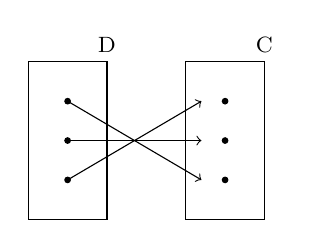
\begin{tikzpicture}
            \draw (0,0) rectangle (1,2) node[above] {\footnotesize D};
            \draw (2,0) rectangle (3,2) node[above] {\footnotesize C};

            \filldraw (0.5, 0.5) circle (1pt);
            \filldraw (0.5, 1) circle (1pt);
            \filldraw (0.5, 1.5) circle (1pt);
            
            \filldraw (2.5, 0.5) circle (1pt);
            \filldraw (2.5, 1) circle (1pt);
            \filldraw (2.5, 1.5) circle (1pt);

            \draw[->] (0.5, 0.5) -- (2.2, 1.5);
            \draw[->] (0.5, 1) -- (2.2, 1);
            \draw[->] (0.5, 1.5) -- (2.2, 0.5);
        \end{tikzpicture}
        &
        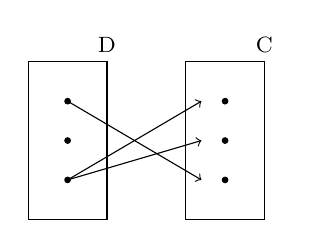
\begin{tikzpicture}
            \draw (0,0) rectangle (1,2) node[above] {\footnotesize D};
            \draw (2,0) rectangle (3,2) node[above] {\footnotesize C};

            \filldraw (0.5, 0.5) circle (1pt);
            \filldraw (0.5, 1) circle (1pt);
            \filldraw (0.5, 1.5) circle (1pt);
            
            \filldraw (2.5, 0.5) circle (1pt);
            \filldraw (2.5, 1) circle (1pt);
            \filldraw (2.5, 1.5) circle (1pt);

            \draw[->] (0.5, 1.5) -- (2.2, 0.5);
            \draw[->] (0.5, 0.5) -- (2.2, 1.5);
            \draw[->] (0.5, 0.5) -- (2.2, 1);
        \end{tikzpicture}
        &
        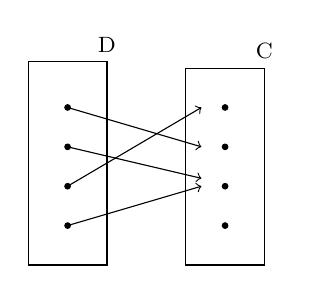
\begin{tikzpicture}
            \draw (0,0) rectangle (1,2.58) node[above] {\footnotesize D};
            \draw (2,0) rectangle (3,2.5) node[above] {\footnotesize C};

            \filldraw (0.5, 0.5) circle (1pt);
            \filldraw (0.5, 1) circle (1pt);
            \filldraw (0.5, 1.5) circle (1pt);
            \filldraw (0.5, 2) circle (1pt);
            
            \filldraw (2.5, 0.5) circle (1pt);
            \filldraw (2.5, 1) circle (1pt);
            \filldraw (2.5, 1.5) circle (1pt);
            \filldraw (2.5, 2) circle (1pt);

            \draw[->] (0.5, 0.5) -- (2.2, 1);
            \draw[->] (0.5, 1) --   (2.2, 2);
            \draw[->] (0.5, 1.5) -- (2.2, 1.1);
            \draw[->] (0.5, 2) -- (2.2, 1.5);
        \end{tikzpicture}
        \\
        Onto? \solution{ yes, every domain element has an input }{} &
        Onto? \solution{ yes, every domain element has an input }{} &
        Onto? \solution{ no, the bottom domain element doesn't have an input }{}
        \\ \notonkey{ \\ }{}
        One-to-one? \solution{ yes, every domain element has max 1 input }{} &
        One-to-one? \solution{ yes, every domain element has max 1 input }{} &
        One-to-one? \solution{ no, one element has 2 inputs }{}
    \end{tabular}
    
\end{question}

\notonkey{ \newpage }{ \hrulefill }

    \section{Isomorphism and Planarity}

    \subsection{Isomorphism}

    \notonkey{
    \begin{intro}{Isomorphism}
        Simple graphs $G$ and $H$ are called \textbf{isomorphic} if there
        is a one-to-one and onto function $f$ from the nodes of $G$ to the nodes of $H$
        such that $\{v, w\}$ is an edge of $G$ if and only if $\{f(v), f(w)\}$
        is an edge of $H$. The function $f$ is called an isomorphism.
        Hence, an isomorphism is simply a \textbf{rule} associating nodes that
        preserves the edges joining the nodes.
        \footnote{Discrete Mathematics, Ensley and Crawley} 

        ~\\
        In other words, two graphs are isomorphic if they're essentially
        the same graph, even if the vertices are in different positions.

        \paragraph{Example:} \tab
        \begin{tabular}{c p{2cm} c}
            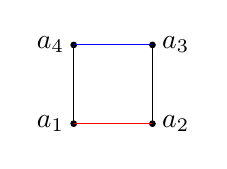
\begin{tikzpicture}
                \filldraw (0,0) circle (1pt) node[left] {$a_{1}$};
                \filldraw (1,0) circle (1pt) node[right] {$a_{2}$};
                \filldraw (1,1) circle (1pt) node[right] {$a_{3}$};
                \filldraw (0,1) circle (1pt) node[left] {$a_{4}$};

                \draw[red] (0,0) -- (1,0);
                \draw (1,0) -- (1,1);
                \draw[blue] (1,1) -- (0,1);
                \draw (0,1) -- (0,0);
            \end{tikzpicture}
            & &
            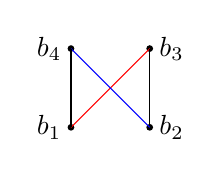
\begin{tikzpicture}
                \filldraw (0,0) circle (1pt) node[left] {$b_{1}$};
                \filldraw (1,0) circle (1pt) node[right] {$b_{2}$};
                \filldraw (1,1) circle (1pt) node[right] {$b_{3}$};
                \filldraw (0,1) circle (1pt) node[left] {$b_{4}$};

                \draw[red] (0,0) -- (1,1);
                \draw (1,0) -- (1,1);
                \draw[blue] (1,0) -- (0,1);
                \draw (0,1) -- (0,0);
            \end{tikzpicture}
            \\ $G$ & & $H$
        \end{tabular}

        These are isomorphic... imagine taking $a_{2}$ and $a_{3}$ from
        graph $G$ and physically flipping them with the edges still connected. In this case,
        our mapping is...
        $a_{1} \to b_{1}$ \tab $a_{2} \to b_{3}$ \tab $a_{3} \to b_{2}$ \tab $a_{4} \to b_{4}$.
    \end{intro}
    }{}

% -------------------------------------------------------------%
% - QUESTION --------------------------------------------------%
% -------------------------------------------------------------%
\stepcounter{question}
\begin{question}{\thequestion}{5}

    Redraw the following graphs by moving the vertices around,
    but keeping the edges connected.

    \begin{itemize}
        \item[a.] 
        \begin{tikzpicture}
            \filldraw (0,0) circle (1pt) node[left] {$a_{1}$};
            \filldraw (2,0) circle (1pt) node[right] {$a_{2}$};
            \filldraw (2,2) circle (1pt) node[right] {$a_{3}$};
            \filldraw (0,2) circle (1pt) node[left] {$a_{4}$};

            \draw (0,0) -- (2,0);
            \draw (2,0) -- (2,2);
            \draw (2,2) -- (0,2);
            \draw (0,2) -- (0,0);
        \end{tikzpicture}
        \solution{
            Example:
            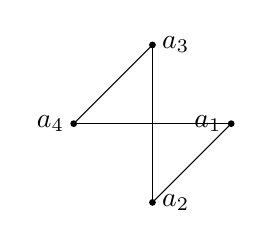
\begin{tikzpicture}
                \filldraw (3,1) circle (1pt) node[left] {$a_{1}$};
                \filldraw (2,0) circle (1pt) node[right] {$a_{2}$};
                \filldraw (2,2) circle (1pt) node[right] {$a_{3}$};
                \filldraw (1,1) circle (1pt) node[left] {$a_{4}$};

                \draw (3,1) -- (2,0);
                \draw (2,0) -- (2,2);
                \draw (2,2) -- (1,1);
                \draw (1,1) -- (3,1);
            \end{tikzpicture}
        }{}

        \item[b.]
        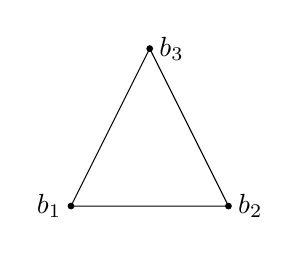
\begin{tikzpicture}
            \filldraw (0,0) circle (1pt) node[left] {$b_{1}$};
            \filldraw (2,0) circle (1pt) node[right] {$b_{2}$};
            \filldraw (1,2) circle (1pt) node[right] {$b_{3}$};

            \draw (0,0) -- (2,0) -- (1,2) -- (0,0);
        \end{tikzpicture}
        \solution{
            Example:
            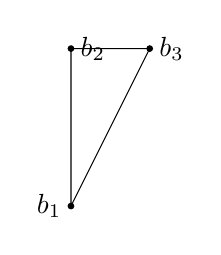
\begin{tikzpicture}
                \filldraw (0,0) circle (1pt) node[left] {$b_{1}$};
                \filldraw (0,2) circle (1pt) node[right] {$b_{2}$};
                \filldraw (1,2) circle (1pt) node[right] {$b_{3}$};

                \draw (0,0) -- (0,2) -- (1,2) -- (0,0);
            \end{tikzpicture}
        }{}
    \end{itemize}

    \solution{
        Multiple solutions...
    }{}
    
\end{question}

\newpage

    \notonkey{
    \begin{intro}{Properties of isomorphic graphs}
        Two graphs that are isomorphic to one another must have...:
        \begin{itemize}
            \item   The same number of nodes
            \item   The same number of edges
            \item   The same number of nodes of any given degree.
            \item   The same number of cycles.
            \item   The same number of cycles of any given size.
        \end{itemize}
        \footnote{Discrete Mathematics, Ensley and Crawley} 
    \end{intro}
    }{}
    
% -------------------------------------------------------------%
% - QUESTION --------------------------------------------------%
% -------------------------------------------------------------%
\stepcounter{question}
\begin{question}{\thequestion}{4}
    % Practice Problem 1
    Given the following two graphs... 

    \begin{center}
        \begin{tabular}{c p{3cm} c}
            G & & H
            \\ \\
            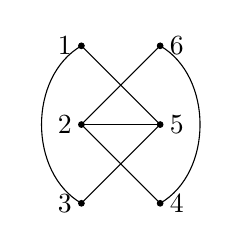
\begin{tikzpicture}
                \filldraw (0,0) circle (1pt) node[left] {3};
                \filldraw (0,1) circle (1pt) node[left] {2};
                \filldraw (0,2) circle (1pt) node[left] {1};
                
                \filldraw (1,0) circle (1pt) node[right] {4};
                \filldraw (1,1) circle (1pt) node[right] {5};
                \filldraw (1,2) circle (1pt) node[right] {6};

                \draw (0,0) -- (1,1) -- (0,2);
                \draw (1,2) -- (0,1) -- (1,0);
                \draw (0,2) to[bend right=60] (0,0);
                \draw (1,0) to[bend right=60] (1,2);
                \draw (0,1) -- (1,1);
            \end{tikzpicture}
            & &
            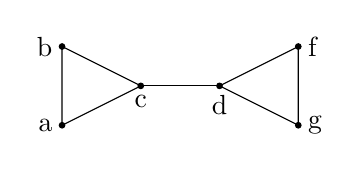
\begin{tikzpicture}
                \filldraw (0,0)     circle (1pt) node[left] {a};
                \filldraw (0,1)     circle (1pt) node[left] {b};
                \filldraw (3,0)     circle (1pt) node[right] {g};
                \filldraw (3,1)     circle (1pt) node[right] {f};
                \filldraw (1,0.5)   circle (1pt) node[below] {c};
                \filldraw (2,0.5)   circle (1pt) node[below] {d};

                \draw (0,0) -- (0,1) -- (1, 0.5) -- (0,0);
                \draw (3,0) -- (3,1) -- (2, 0.5) -- (3,0);
                \draw (1,0.5) -- (2,0.5);
            \end{tikzpicture}
        \end{tabular}        
    \end{center}

    \begin{itemize}
        \item[a.]   Write out all edges for both graphs.

            $G$: \{2, 5\}
                     \solution{ \{ 2, 3 \} }{}
                     \solution{ \{ 3, 4 \} }{}
                     \solution{ \{ 4, 5 \} }{}
                     \solution{ \{ 2, 5 \} }{}
                     \solution{ \{ 5, 6 \} }{}

            $H$: \{d, c\}
                     \solution{ \{ y, x \} }{}
                     \solution{ \{ x, w \} }{}
                     \solution{ \{ w, v \} }{}
                     \solution{ \{ y, v \} }{}
                     \solution{ \{ v, u \} }{}

        \item[b.]   For each edge from $G$, write out what edge in $H$ corresponds to it.
            \tab Example: \{2,5\} $\to$ \{d, c\} \\
            
            \solution{
                Let's split up $G$ into two subgraphs to see it more clearly...
                
                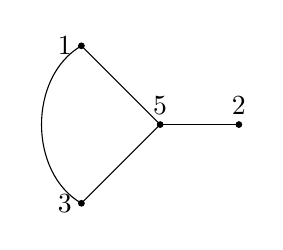
\begin{tikzpicture}
                    \filldraw (0,0) circle (1pt) node[left] {3};
                    \filldraw (0,2) circle (1pt) node[left] {1};
                    \filldraw (1,1) circle (1pt) node[above] {5};
                    \filldraw (2,1) circle (1pt) node[above] {2};
                    \draw (0,0) -- (1,1) -- (0,2);
                    \draw (0,2) to[bend right=60] (0,0);
                    \draw (1,1) -- (2,1);
                \end{tikzpicture}  \tab 
                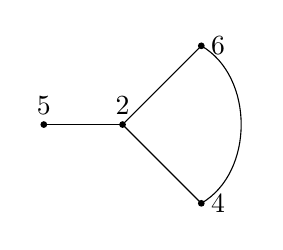
\begin{tikzpicture}                    
                    \filldraw (-1,1) circle (1pt) node[above] {5};
                    \filldraw (0,1) circle (1pt) node[above] {2};
                    \filldraw (1,0) circle (1pt) node[right] {4};
                    \filldraw (1,2) circle (1pt) node[right] {6};

                    \draw (1,2) -- (0,1) -- (1,0);
                    \draw (1,0) to[bend right=60] (1,2);
                    \draw (0,1) -- (-1,1);
                \end{tikzpicture}
            
                $\{1,3\} \to \{b, a\}$ \tab
                $\{1,5\} \to \{b, c\}$ \tab
                $\{2,4\} \to \{d, e\}$ \\
                $\{2,5\} \to \{d, c\}$ \tab
                $\{2,6\} \to \{d, f\}$ \tab
                $\{3,5\} \to \{a, c\}$ \\
                $\{4,6\} \to \{e, f\}$
            }{}
    \end{itemize}
    
\end{question}
    
\newpage

    \subsection{Adjacency matrix}

    \begin{intro}{\ }
        We can also use a matrix to list out which vertices are adjacent
        to which other vertices in order to help us figure out if two
        graphs are isomorphic.

        \paragraph{Example:} ~\\

        \begin{tabular}{p{6cm} p{6cm}}
        
            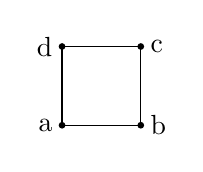
\begin{tikzpicture}
                \filldraw (0,0) circle (1pt) node[left] {a};
                \filldraw (1,0) circle (1pt) node[right] {b};
                \filldraw (1,1) circle (1pt) node[right] {c};
                \filldraw (0,1) circle (1pt) node[left] {d};

                \draw (0,0) -- (1,0) -- (1,1) -- (0,1) -- (0,0);
            \end{tikzpicture}

            &

            \begin{tabular}{c | c c c c}
                & a & b & c & d
                \\ \hline
                a & 0 & \textbf{1} & 0 & \textbf{1}
                \\
                b & \textbf{1} & 0 & \textbf{1} & 0
                \\
                c & 0 & \textbf{1} & 0 & \textbf{1}
                \\
                d & \textbf{1} & 0 & \textbf{1} & 0
            \end{tabular}
            
        \end{tabular}

        $a$ is adjacent to $b$ and $d$, so in the $a$ row we have 1's under the $b$ and $d$ columns.
    \end{intro}

% -------------------------------------------------------------%
% - QUESTION --------------------------------------------------%
% -------------------------------------------------------------%
\stepcounter{question}
\begin{question}{\thequestion}{4}

    For the following graph...

    \begin{center}
        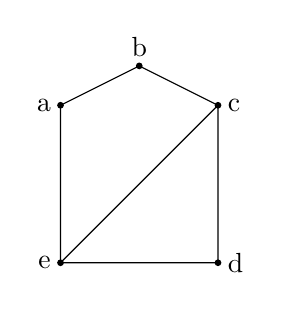
\begin{tikzpicture}
            \filldraw (0,0) circle (1pt) node[left]         {e};
            \filldraw (2,0) circle (1pt) node[right]        {d};
            \filldraw (2,2) circle (1pt) node[right]        {c};
            \filldraw (0,2) circle (1pt) node[left]         {a};
            \filldraw (1,2.5) circle (1pt) node[above]    {b};

            \draw (0,0) -- (2,0) -- (2,2) -- (1,2.5) -- (0,2) -- (0,0) -- (2,2);
        \end{tikzpicture}
    \end{center}

    \begin{itemize}
        \item[a.]   Finish the adjacency matrix: \tab
            \begin{tabular}{c | c | c | c | c | c}
                & a & b & c & d & e
                \\ \hline
                a
                    & \solution{0}{}
                    & \solution{1}{}
                    & \solution{0}{}
                    & \solution{0}{}
                    & \solution{1}{}
                \\ \hline
                b
                    & \solution{1}{}
                    & \solution{0}{}
                    & \solution{1}{}
                    & \solution{0}{}
                    & \solution{0}{}
                \\ \hline
                c
                    & \solution{0}{}
                    & \solution{1}{}
                    & \solution{0}{}
                    & \solution{1}{}
                    & \solution{1}{}
                \\ \hline
                d
                    & \solution{0}{}
                    & \solution{0}{}
                    & \solution{1}{}
                    & \solution{0}{}
                    & \solution{1}{}
                \\ \hline
                e
                    & \solution{1}{}
                    & \solution{0}{}
                    & \solution{1}{}
                    & \solution{1}{}
                    & \solution{0}{}
            \end{tabular}
        ~\\~\\
        \item[b.]   Fill out the degrees of each:
            \begin{tabular}{ p{1cm} |p{1cm} |p{1cm} |p{1cm} |p{1cm} }
                a & b & c & d & e
                \\ \hline
                  \solution{ 2 }{} % a
                &   \solution{ 2 }{} % b
                &   \solution{ 3 }{} % c 
                &   \solution{ 2 }{} % d
                &   \solution{ 3 }{} % e
                \\
                & & & & \\
            \end{tabular}
    \end{itemize}
    
\end{question}

\newpage

    \subsection{Planarity}

    \begin{introNOHEAD}{}
        \begin{enumerate}
            \item   A simple, connected graph is called \textbf{planar}
                    if there is a way to draw it (on a plane) so that
                    no edges cross (i.e., they can only meet at a node).
                    We will call ``drawing" of a graph on a plane
                    surface with no edge-crossings an \textbf{embedding}
                    of the graph in the plane.

            \item   A graph is called \textbf{bipartite} if its set of nodes
                    can be partitioned into two disjoint sets $S_{1}$
                    and $S_{2}$ so that every edge in the graph has one
                    endpoint in $S_{1}$ and one endpoint in $S_{2}$.

            \item   The \textbf{complete graph} on $n$ nodes, denoted
                    by $K_{n}$, is the simple graph with nodes
                    $\{1, ..., n\}$ and an edge between every pair of distinct nodes.

            \item   The \textbf{complete bipartite graph} on $n,m$ nodes,
                    denoted by $K_{n,m}$, is the simple bipartite graph
                    with nodes $S_{1} = \{a_{1}, a_{2}, ..., a_{n}\}$ and
                    $S_{2} = \{b_{1}, b_{2}, ..., b_{m}\}$ and
                    with edges connecting each node in $S_{1}$ to every
                    node in $S_{2}$.
        \end{enumerate}
        \footnote{Discrete Mathematics, Ensley and Crawley}

        \paragraph{Example:}
        Let's redraw the graph $K_{4}$ so it has no overlapping edges.

        \begin{center}
            \begin{tabular}{c p{3cm} c}
                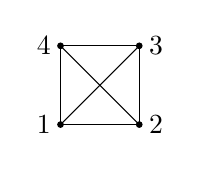
\begin{tikzpicture}
                    \filldraw (0,0) circle (1pt) node[left]     {1};
                    \filldraw (0,1) circle (1pt) node[left]     {4};
                    \filldraw (1,0) circle (1pt) node[right]    {2};
                    \filldraw (1,1) circle (1pt) node[right]    {3};

                    \draw (0,0) -- (1,0) -- (1,1) -- (0,1) -- (0,0);
                    \draw (0,0) -- (1,1);
                    \draw (1,0) -- (0,1);
                \end{tikzpicture}
                & &
                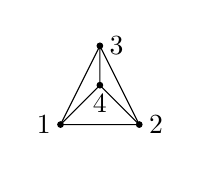
\begin{tikzpicture}
                    \filldraw (0,0) circle (1pt) node[left]     {1};
                    \filldraw (0.5,0.5) circle (1pt) node[below]     {4};
                    \filldraw (1,0) circle (1pt) node[right]    {2};
                    \filldraw (0.5,1) circle (1pt) node[right]    {3};

                    \draw (0,0) -- (1,0) -- (0.5,1) -- (0.5,0.5) -- (0,0);
                    \draw (0,0) -- (0.5,1);
                    \draw (1,0) -- (0.5,0.5);
                \end{tikzpicture}
                \\
                $K_{3}$ & & $K_{3}$ redrawn
            \end{tabular}
        \end{center}
    \end{introNOHEAD}
    
% -------------------------------------------------------------%
% - QUESTION --------------------------------------------------%
% -------------------------------------------------------------%
\stepcounter{question}
\begin{question}{\thequestion}{2}

    % Example 4
    Redraw the following graph, $K_{3,2}$, so that no edges are overlapping.

    ~\\~\\
    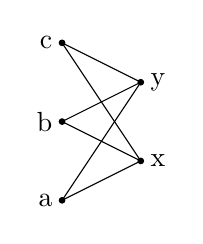
\begin{tikzpicture}
        \filldraw (0,0) circle (1pt) node[left]         {a};
        \filldraw (0,1) circle (1pt) node[left]         {b};
        \filldraw (0,2) circle (1pt) node[left]         {c};
        \filldraw (1,0.5) circle (1pt) node[right]         {x};
        \filldraw (1,1.5) circle (1pt) node[right]         {y};
        \draw (0,0) -- (1,0.5) -- (0,1) -- (1,1.5) -- (0,2) -- (1,0.5);
        \draw (0,0) -- (1,1.5);
    \end{tikzpicture}
    \solution{
        Example:
        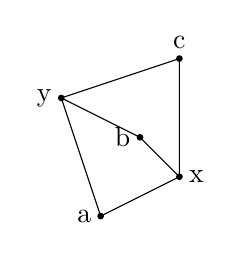
\begin{tikzpicture}
            \filldraw (0,0) circle (1pt) node[left]         {a};
            \filldraw (0.5,1) circle (1pt) node[left]         {b};
            \filldraw (1,2) circle (1pt) node[above]         {c};
            \filldraw (1,0.5) circle (1pt) node[right]         {x};
            \filldraw (-0.5,1.5) circle (1pt) node[left]         {y};
            \draw (0,0) -- (1,0.5) -- (0.5,1) -- (-0.5,1.5) -- (1,2) -- (1,0.5);
            \draw (0,0) -- (-0.5,1.5);
        \end{tikzpicture}
    }{}
                
\end{question}


    \begin{intro}{Faces}
        For a planar graph $G$ embedded in the plane,
        a \textbf{face} of the graph is a region of the plane created
        by the drawing. Since the plane is an unbounded surface, every
        embedding of a finite planar graph will have exactly one
        \textbf{unbound} face.
        \footnote{Discrete Mathematics, Ensley and Crawley}

        \paragraph{Unbound (external) face:}
        Think of the external face as the ``canvas" that all other
        faces are painted on to. Or, if you were viewing a silhouette of
        the drawing, you would only see the unbounded face - the sum of
        all the faces.
        % I legit cannot find a proper definition for "unbounded face"
        % online or in the book, wtf.

        \begin{wrapfigure}{r}{0.3\textwidth}
            \begin{center}
                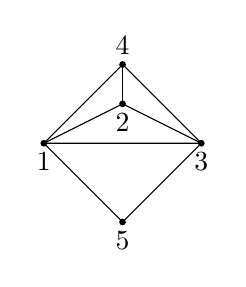
\begin{tikzpicture}
                    \filldraw (0,0) circle (1pt) node[below]{5};
                    \filldraw (-1,1) circle (1pt) node[below]{1};
                    \filldraw (1,1) circle (1pt) node[below]{3};
                    \filldraw (0,1.5) circle (1pt) node[below]{2};
                    \filldraw (0, 2) circle (1pt) node[above]{4};

                    \draw (-1,1) -- (1,1) -- (0,0) -- (-1,1);
                    \draw (-1,1) -- (0,1.5) -- (1,1);
                    \draw (-1,1) -- (0,2);
                    \draw (1,1) -- (0,2);
                    \draw (0,1.5) -- (0,2);
                \end{tikzpicture}
            \end{center}
        \end{wrapfigure}
        
        \paragraph{Example:} ~\\
            For the drawing, identify the faces by giving the cycle that
            creates each face, and highlight the unbounded face.

        ~\\
        Faces: ~\\
        \begin{tabular}{c c c}
            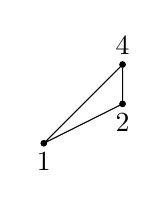
\begin{tikzpicture}
                \draw (-1,1) -- (0,1.5) -- (0,2) -- (-1,1);
                \filldraw (-1,1) circle (1pt) node[below]{1};
                \filldraw (0,1.5) circle (1pt) node[below]{2};
                \filldraw (0, 2) circle (1pt) node[above]{4};
            \end{tikzpicture}  &
            
            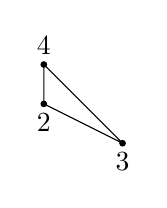
\begin{tikzpicture}
                \draw (1,1) -- (0,1.5) -- (0,2) -- (1,1);
                \filldraw (1,1) circle (1pt) node[below]{3};
                \filldraw (0,1.5) circle (1pt) node[below]{2};
                \filldraw (0, 2) circle (1pt) node[above]{4};
            \end{tikzpicture} \\

            1, 2, 4, 1 & 2, 3, 4, 2 \\
            
            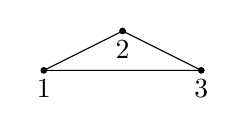
\begin{tikzpicture}
                \draw (-1,1) -- (1,1) -- (0, 1.5) -- (-1,1);
                \filldraw (-1,1) circle (1pt) node[below]{1};
                \filldraw (1,1) circle (1pt) node[below]{3};
                \filldraw (0,1.5) circle (1pt) node[below]{2};
            \end{tikzpicture}  &
            
            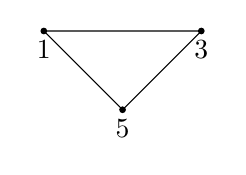
\begin{tikzpicture}
                \draw (-1,1) -- (1,1) -- (0,0) -- (-1,1);
                \filldraw (0,0) circle (1pt) node[below]{5};
                \filldraw (-1,1) circle (1pt) node[below]{1};
                \filldraw (1,1) circle (1pt) node[below]{3};
            \end{tikzpicture} &
            
            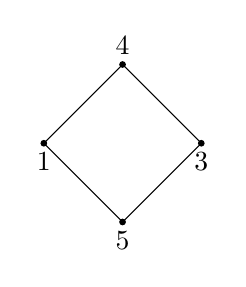
\begin{tikzpicture}
                \draw (-1,1) -- (0,0) -- (1,1) -- (0,2) -- (-1,1);
                \filldraw (0,0) circle (1pt) node[below]{5};
                \filldraw (-1,1) circle (1pt) node[below]{1};
                \filldraw (1,1) circle (1pt) node[below]{3};
                \filldraw (0, 2) circle (1pt) node[above]{4};
            \end{tikzpicture}

            \\ 1, 2, 3, 1 & 1, 3, 5, 1 & 1, 4, 3, 5, 1
            \\ & & (unbounded)
            
        \end{tabular}

    \end{intro}

\newpage

% -------------------------------------------------------------%
% - QUESTION --------------------------------------------------%
% -------------------------------------------------------------%
\stepcounter{question}
\begin{question}{\thequestion}{2}
    
    For both graphs, draw out each of its \textbf{faces}, then
    write out all the cycles bordering faces and identify the unbounded cycle.

    \begin{itemize}
        \item[a.]
            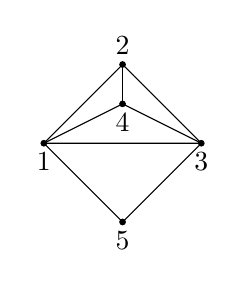
\begin{tikzpicture}
                \filldraw (0,0) circle (1pt) node[below]{5};
                \filldraw (-1,1) circle (1pt) node[below]{1};
                \filldraw (1,1) circle (1pt) node[below]{3};
                \filldraw (0,1.5) circle (1pt) node[below]{4};
                \filldraw (0, 2) circle (1pt) node[above]{2};

                \draw (-1,1) -- (1,1) -- (0,0) -- (-1,1);
                \draw (-1,1) -- (0,1.5) -- (1,1);
                \draw (-1,1) -- (0,2);
                \draw (1,1) -- (0,2);
                \draw (0,1.5) -- (0,2);
            \end{tikzpicture}

        \solution{
            1, 2, 4, 1 \tab 1, 3, 5, 1 \tab 2, 3, 4, 2 \\
            1, 3, 4, 1 \tab 1, 2, 3, 5, 1 (unbounded).
        }{}
        ~\\~\\
        \item[b.]
            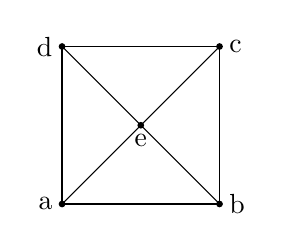
\begin{tikzpicture}
                \filldraw (0,0) circle (1pt) node[left]{a};
                \filldraw (2,0) circle (1pt) node[right]{b};
                \filldraw (2,2) circle (1pt) node[right]{c};
                \filldraw (0,2) circle (1pt) node[left]{d};
                \filldraw (1,1) circle (1pt) node[below]{e};

                \draw (0,0) -- (2,0) -- (2,2) -- (0,2) -- (0,0);
                \draw (0,0) -- (1,1) -- (0,2);
                \draw (2,0) -- (1,1) -- (2,2);
            \end{tikzpicture}

            \solution{
                a, b, e, a  \tab    a, e, d, a  \tab d, e, c, d \tab b, c, e, b
                \\
                a, b, c, d, a (unbounded)
            }{}
    \end{itemize}
    
\end{question}



\end{document}
